%%%%%%%%%%%%%%%%%%%%%%%%%%%%%%%%%%%%%%%%%%%%%%%%%%%%%%%%%%%%%%%%%%%%%%%%%%%
% Copyright (c) 2010 committers of YAKINDU and others.
% All rights reserved. This program and the accompanying materials
% are made available under the terms of the Eclipse Public License v1.0
% which accompanies this distribution, and is available at
% http://www.eclipse.org/legal/epl-v10.html
%
% Contributors:
%     committers of YAKINDU - initial API and implementation
%%%%%%%%%%%%%%%%%%%%%%%%%%%%%%%%%%%%%%%%%%%%%%%%%%%%%%%%%%%%%%%%%%%%%%%%%%%
\section{Introduction}
In our previous examples we created a YAKINDU state chart with the YAKINDU
Statechart Editor. However, it is also possible to import an existing UML2
state machine or create one with your favourite UML2 tool (You may also use
the UML2 Editor which ships with the eclipse modelling distribution). The tool
of your choice must support "EMF UML2". In our examples we are going to use
the UML2-Toools available in Galileo.

If you want to use an UML2 modelling tool instead of the YAKINDU Statechart
Editor or you have an existing UML2 state machine, you need to consider that
the YAKINDU state charts are somehow different from the UML2 state machines.
To fill this gap you have to extend your UML2 state machine (In future
releases another approach may also be available).

%or, if this is not anoption, you can create extensions for the transformation.

\section{UML2 model}
As for the code genenerators, an example project for transformation of UML2
state machines to YAKINDU state charts is also available. You can open the
examples (see Figure \ref{fig:uml2tools}) and compare them with the generated
YAKINDU state charts. \begin{figure}[ht]
\center
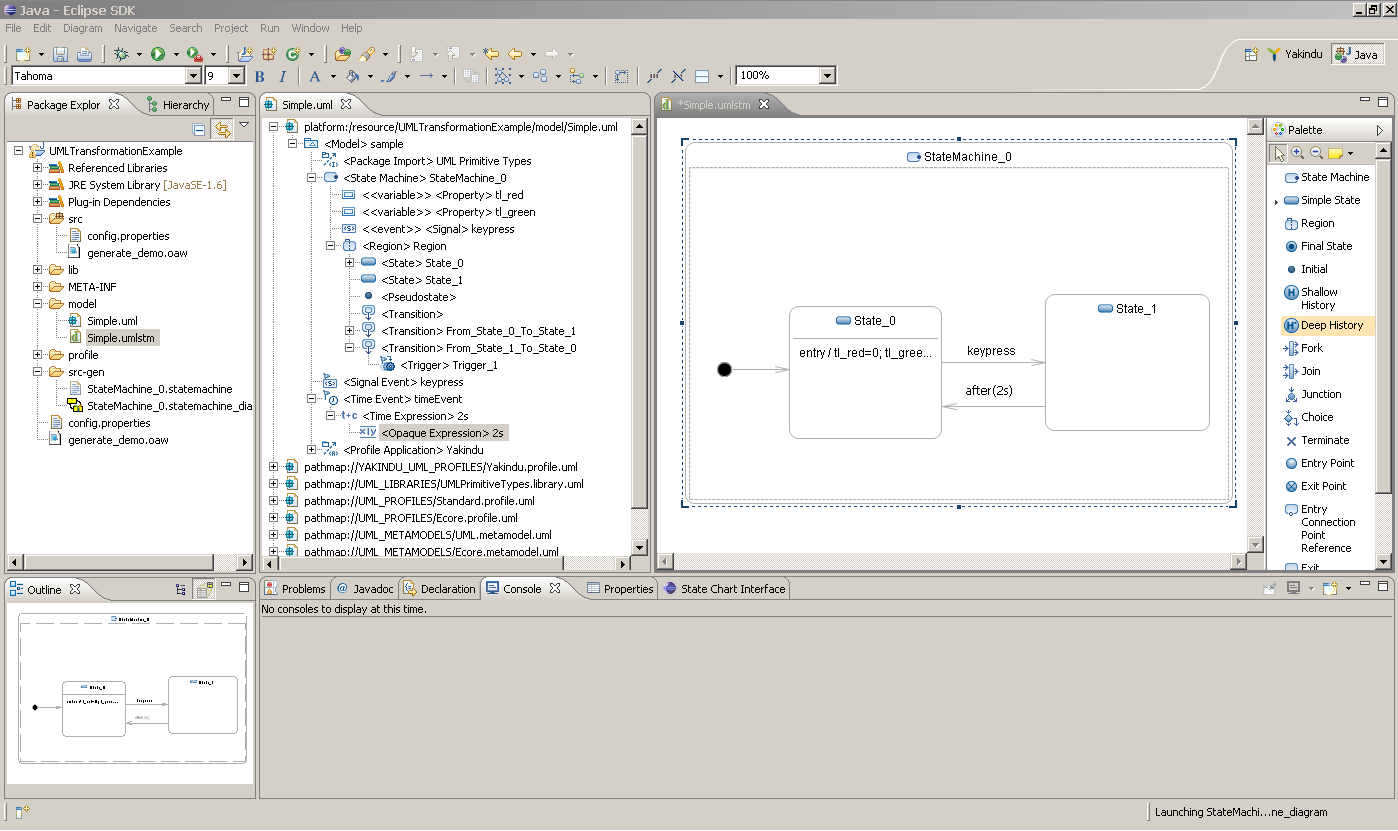
\includegraphics[width=1\textwidth]{Pictures/uml2tools}
\caption{\label{fig:uml2tools}UML2 state machine in eclipse} 
\end{figure}

Some information, which cannot be modelled in UML2 are generated
automatically, or as mentioned before, can be specified somehow else. For
example: Every Transition and every Region in a YAKINDU state chart needs a
priority. On how to set a priority will be discussed later. Lets have a look
at an example project first.

\section{The example project}
The example is available within eclipse under \textbf{File} $\rightarrow$
\textbf{New} $\rightarrow$ \textbf{Example\dots} within the category
\textbf{YAKINDU Examples}. Select ''UML -> YAKINDU Transformation'' and Finish the
dialog. A new project ''UML\_TransformationExample'' containing one UML
diagrams inclusive ''.umlstm'' diagram file for UML tools will be created.

\begin{floatingfigure}[r]{0.3\textwidth}
  \centering
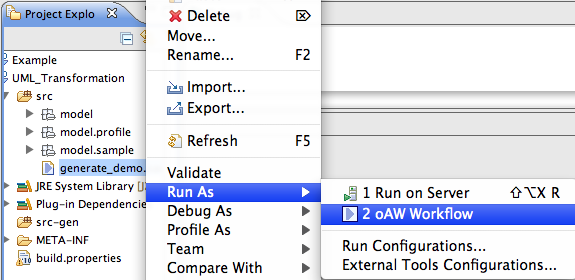
\includegraphics[width=0.3\textwidth]{Pictures/runTransformationUMLAs}
\caption{\label{fig:runTransformationUMLAs}Run UML transformation workflow} 
\end{floatingfigure}
To generate the YAKINDU state chart, right-click on
\textbf{generate\_demo.oaw} and select \textbf{Run As} $\rightarrow$
\textbf{MWE Workflow} (Compare Figure \ref{fig:runTransformationUMLAs}). The
output of the transformation is saved in the new folder src-gen and the status
of the run is available in the Console view of eclipse, which will be
automatically opened in the right corner at the bottom of the window.

The result is a *.statemachine file which can be found in the src-gen folder
within your project. The output folder, where your statemachines will be generated
and the UML2 model can be defined in the generatordemo.oaw. The next step,
which should follow, is to generate a diagram for your model. This is not
automatically done, but with a right-click on the statemachine file you can
initialize a diagram (see figure \ref{fig:initializeDiagram}). Because the
layout information are not stored inside UML2 you have to draft your diagram
by hand. \begin{figure}[ht]
\center
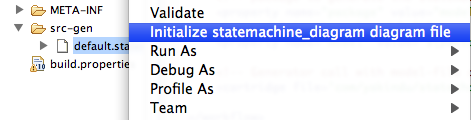
\includegraphics[width=0.6\textwidth]{Pictures/initializeDiagram}
\caption{\label{fig:initializeDiagram}Initialize Diagram} 
\end{figure}

The generated state chart can be edited, simulated and code can be generated
from it. These steps were described in previous chapters. If you want to
generate code from the state chart see Chapter \ref{sec:CCodeGenerator} for C
and Chapter \ref{sec:JavaCodeGenerator} for Java. If the model is a valid
YAKINDU state chart a simulation is also possible (see Chapter
\ref{sec:simulatingStateMachine}).

\section{How does it work}
The UML2 state machine and the YAKINDU state chart are quite similar.
Nevertheless, there are a few differences that need to be cared of.

\subsection{Name mapping}
The naming is the smallest gap. The following table shows the name mapping
between the UML2 state machine and the YAKINDU state chart.

\begin{table}[ht]
\begin{center}
\begin{tabular}{|c|c|}
\hline UML2 & YAKINDU \\
\hline
StateMachine & Statechart \\
Region & Region \\
Transition & Transition \\
Vertex & Node \\
State &  State \\
FinalState & FinalState \\
Pseudostate & Pseudostate \\
\hline
\end{tabular}
\end{center}
\caption{UML2 - YAKINDU Mapping}
\label{UML2 - YAKINDU Mapping}
\end{table}

As you can see, there are only marginal differences. Besides that, YAKINDU state
chart also defines new elements which are not present in the UML2.

\subsection{New elements}
The new elements are Variable and Event. As those can't be mapped 1:1, some
conventions are needed. The default behavior of the transformation is to ignore
those elements. This will result in an incomplete YAKINDU state chart (therefore
no simulation is possible). To %prevent this, you can decide between two methods.
prevent this, you have to extend your UML2 state machine.

\subsection{Limitations}
There are a few UML Elements that are currently not supported by the transformation. That includes the
PseudoStates
\begin{itemize}
\item join
\item fork
\item entryPoint
\item exitPoint
\item and terminate.
\end{itemize}
A transformation that encounters such
an element will fail.

\subsection{Transformation Cartridge}
The Transformation Cartridge allows you to integrate the YAKINDU Transformation into
your oAW Workflow. The cartridge expects the following parameters.

\begin{table}[ht]
\begin{center}
\begin{tabular}{|l|l|}
\hline Parameter & Description \\
\hline
umlModel & A path to your UML2 Model file. \\
srcgen &  The output folder where the generated *.statemachine files should be created. \\
package &  The root directory for the transformation. \\
\hline
\end{tabular}
\end{center}
\caption{YAKINDU Transformation Cartridge Parameters}
\label{YAKINDU Transformation Cartridge Parameters}
\end{table}

In your oAW Workflow it may look like this:\begin{verbatim}
...
<property name="umlModel" value="model/Simple.uml"/>
<property name="src-gen" value="src-gen"/>
<property name="config" value="src/" />

<!-- Generator call with model-file and output-folder -->
<cartridge file='com/yakindu/statechart/transformation/uml2/transform.oaw' 
	project="com.yakindu.statechart.transformation.examples.uml2"
 	umlModel="${umlModel}" 
 	src-gen="${src-gen}" 
 	config="${config}" />
...
\end{verbatim} 


\section{Extending an UML2 state machine}
% The first method is to modify your UML2 state machine.
Since there aren't UML2 Elements called Variable or Event, those have to be
created with the existing UML2 elements and the YAKINDU UML2 profile. The profile
allows you to give Transitions and Regions a priority and to describe Events as
Signals and Variables as Classes.

First you need to apply the YAKINDU UML2 profile.  Open your *.uml file and select the model.
Click on \textbf{UML Editor} $\rightarrow$ \textbf{Package} $\rightarrow$
\textbf{Apply Profile}. A new window pops up where you add the YAKINDU UML2
profile to your model. Press \textbf{Ok} and save the *.uml file. Now that the
profile has been loaded you need to apply the stereotypes to various elements.
You can do this with the UML Editor which has been used until now.
\begin{figure}[h!]
\center
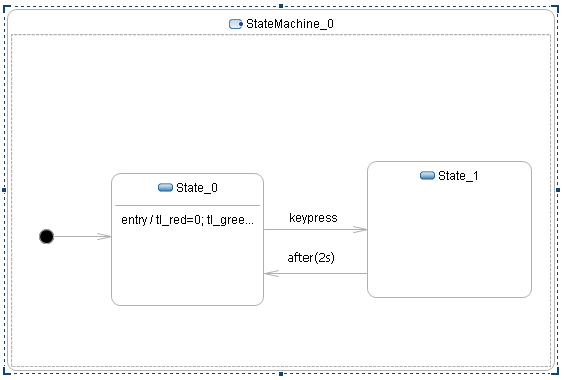
\includegraphics[width=0.5\textwidth]{Pictures/priorityVisualisation}
\caption{\label{fig:priorityVisualisation}UML2 state machine example} 
\end{figure}

Open the related *.umlstm file. It should look somehow like Figure
\ref{fig:priorityVisualisation}. The YAKINDU UML2 profile allows us to apply the
stereotypes Priority, Variable and Event. Priority can be applied to Transitions
and Regions, Variable to Classes and Event to Signals. First, we want to give
every Transition and every Region a Priority. To do so, select a
Transition/Region in the UML Editor. Select \textbf{UML Editor} $\rightarrow$ \textbf{Element} $\rightarrow$
\textbf{Apply Stereotype\dots}. Afterwards you can edit the priority in the properties tab, if element is selected.
\begin{figure}[h!] \center
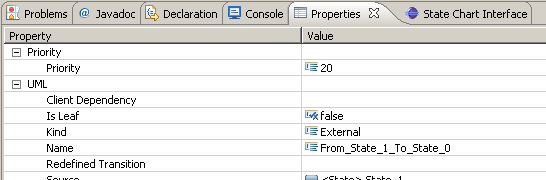
\includegraphics[width=0.9\textwidth]{Pictures/changePriority}
\caption{\label{fig:changePriority}Change the Priority} 
\end{figure}
The default value for Priority is 0 (see figure
\ref{fig:changePriority}). That's it! Repeat this for every Transition/Region in
your State machine.

Now we are going to add the Stereotypes Event to our Signals. Most work will be done in the tree UML Editor. 
\begin{figure}[h] \center
\includegraphics[width=0.9\textwidth]{Pictures/editorApplyStereotype}
\caption{\label{fig:editorApplyStereotype}Apply Stereotype} 
\end{figure}

Select a Signal and click on \textbf{UML Editor} $\rightarrow$ \textbf{Element}
$\rightarrow$\textbf{Apply Stereotype} (see figure
\ref{fig:editorApplyStereotype}). Add YAKINDU::Event and press \textbf{OK}. In
the Properties View you can see now a Property Event with some Attributes.
\begin{figure}[h] 
\center
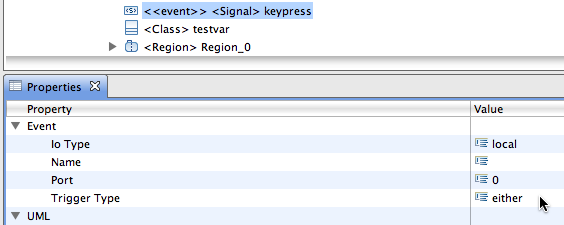
\includegraphics[width=0.9\textwidth]{Pictures/editorProperty}
\caption{\label{fig:editorProperty}Change Attributes} 
\end{figure}
Change those Attributes to your needs (see figure \ref{fig:editorProperty}).
Repeat this for every Signal in your state machine.

To add Variables to your UML2 state machine you have to create properties for your variable first. 
\begin{figure}[h] 
\center
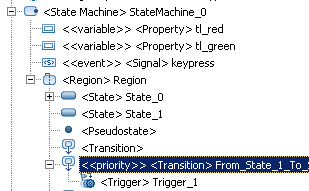
\includegraphics[width=0.7\textwidth]{Pictures/variableExpression}
\caption{\label{fig:variableExpression}Property named after a Variable} 
\end{figure}

Those have to be named after the Variables in the Expressions of your Transitions
(see figure \ref{fig:variableExpression}). If you created a Property, select it and click
on \textbf{UML Editor} $\rightarrow$ \textbf{Element} $\rightarrow$
\textbf{Apply Stereotype}. Add YAKINDU::Variable and press \textbf{OK}. In the
Properties View you can change now the Attributes of Variable to your needs.
Repeat this for every Variable in you Expressions.

It is important to know that Signals and Properties that should be recognized as Events
and Variables must be created under the state machine in the UML2 model. This is
necessary due to the fact that any number of state machines can be in a UML2 model.

If you followed all the described steps you are now able to generate a valid
YAKINDU state chart.


%(ok)- how to use the transformation by example
%- how to simulate a transformed model
%(code?)- how to generate from a transformed model
%- how the transformation works (important mapping rules)
%-> Role of clasifier/class
%-> (done) using the profile
%-> (not yet) using alternatives to the profile


\clearpage